\documentclass[Japanese]{dicomopapers}
%\documentclass[Japanese,noauthor]{dicomopapers}

\usepackage[dvips]{graphicx}
\usepackage{latexsym}

\def\Underline{\setbox0\hbox\bgroup\let\\\endUnderline}
\def\endUnderline{\vphantom{y}\egroup\smash{\underline{\box0}}\\}
\def\|{\verb|}

\begin{document}

% 和文表題
\title{IoTデバイスの通信セキュリティ向上のための\\ホームネットワーク仮想化フレームワークの提案}
% 英文表題
\etitle{Proposal of Home Network Virtualization Framework\\to Improve Communication Security of IoT Devices}

% 所属ラベルの定義
\affiliate{DOSHISHA}{同志社大学大学院 理工学研究科\\Graduate School of Science and Engineering, Doshisha University}
\affiliate{MOBILITY}{同志社大学モビリティ研究センター\\Mobility Reserch Center, Doshisha University}

\author{塚崎 拓真}{TAKUMA TSUKASAKI}{DOSHISHA}
\author{滕 睿}{RUI TENG}{MOBILITY}
\author{佐藤 健哉}{KENYA SATO}{DOSHISHA}

\begin{abstract}
	近年,IoT(Internet of Things)が注目を集めるようになり,今後あらゆるモノがネットワークに接続され,利用されることが予想される.しかし,IoTの発展により利便性が高まる一方で,これまでネットワークに接続されていなかったモノが接続されることにより,セキュリティ上のリスクも高まっている.また,今後はホームネットワーク内で閉じたデバイス間の通信によって連携を行う形になることが想定される.デバイス間で直接通信を行う場合,各デバイスにおいてどのデバイスとの通信を受け入れるか,アクセス制御を行う必要がある.そこで本研究では,SDN(Software Defined Networks)の代表的プロトコルであるOpenFlowを用いて,ホームネットワーク内の通信を監視するフレームワークの構築を検討した.また,提案システムでは,セキュリティ対策を適用可能なProxyを仮想的に作成した.このProxyにセキュリティ対策をオフロードし,IoTデバイス間の通信を中継することで,本来IoTデバイスに適用したいセキュリティ対策を実現した.そして,IoTデバイス間で閉じた通信を行うシミュレーションの評価を行い,ホームネットワークにおいてセキュリティ要件を保つことを示した.

\end{abstract}

% 表題などの出力
\maketitle

% 本文はここから始まる
\section{はじめに}
近年,IoT(Internet of Things)が注目を集めるようになり,今後あらゆるモノがネットワークに接続され,利用されることが予想される.
あらゆるモノがIoTによりネットワークに接続されることで、情報流通を促進し、ビッグデータを収集、解析が行われることに加え、ローカルネットワーク内においても、今後様々なIoTデバイスの登場により、今まで相互接続されていなかった機器同士が接続されると考えられる.以上のような変化により、様々な課題の解決や新たな価値の創出が期待されている.\par
しかし,IoTの発展により利便性が高まる一方で,これまでネットワークに接続されていなかったモノが接続されることにより,セキュリティ上のリスクも高まっている\cite{security}.
IoTデバイスは十分なセキュリティを考慮せずに開発されたものが多いため,悪意のある攻撃者によるサイバー攻撃の標的になりやすい.
脅威としては、ホームネットワークに侵入し、デバイスの遠隔操作による外部サーバへの攻撃やマルウェア感染によるプライバシーに関わる機密情報の収集などが挙げられる.
また、攻撃によってホームネットワーク内に侵入されてしまうと、その内部でも端末間で自由にアクセス可能なため、マルウェア感染などのリスクがホームネットワーク全体の端末に広がる可能性がある.したがって、ホームネットワークのセキュリティ対策として、侵入を前提に攻撃を受けた時に被害を最小化できることが重要である.
% また,現在のスマートホームデバイスは,クラウド上のシステムと連携することで,デバイス間の連携を可能にしているが,今後はホームネットワーク内で閉じたデバイス間の通信によって連携を行う形になることが想定される.
% デバイス間で直接通信を行う場合,各デバイスにおいてどのデバイスとの通信を受け入れるか,アクセス制御を行う必要がある.
% セキュリティ上の脅威が各種デバイスに顕在した場合,個別に対処するとコストや時間がかかってしまうため,脅威に対し一括に対処する必要がある.\par
% しかし,ホームネットワーク内には異なる規格のハードウェアや様々なアプリケーションが混在しているため,それら全てに対応したシステムの構築や更新を続けるのは困難である.
% しかし,全てのデバイスがアクセス制御に対応しているとは限らず,デバイスの計算能力の制限によって実現できるアクセス制御に制限がある場合や,デバイスのソフトウェア自体の脆弱性によってアクセス制御が機能しない場合が考えられる.
しかし、IoTデバイスは従来のPC等の既存機器と比較した場合,CPU等のリソースを十分に保持していないため,デバイスの計算能力の制限やソフトウェア自体の脆弱性によって,適用できる機能が限られるという問題がある.
そのため、暗号化等のセキュリティ対策の適用は困難となり、どのデバイスも必ず利用するネットワークを利用したシステムを構築することや仮想的に作成したシステムを構築することが望ましい.\par
そこで本研究では,SDN(Software Defined Networks)の代表的プロトコルであるOpenFlow\cite{openflow}を用いて,ホームネットワーク内の通信を監視し、また、セキュリティ対策を施し仮想的に作成したProxyを利用し、IoTデバイスに対してセキュリティ対策を施すフレームワークの構築を検討した.
% OpenFlowを利用することで,既存IoTデバイスや異なる規格などに対応でき,ホームネットワークに適した形で不正な通信の検知を実現する.
% また,提案システムでは,セキュリティ対策を適用可能なデバイスをProxyと定義し,ルータ内に配置されたコンテナ内に仮想的に作成する.
% ここに,IoTデバイスがリソース量の制限により適用できないセキュリティ対策をオフロードし,このProxyがIoTデバイス間の通信を中継することで,本来IoTデバイスに適用したいセキュリティ対策を実現する.
% セキュリティ対策として,ホームネットワーク内の通信のトラフィック情報は既知であることを考慮し,フローの検証をOpenFlowコントローラで行う.\par
% ルータ内にコンテナを配置し,そのコンテナ上にProxyを作成する.そして,IoTデバイス間で閉じた通信を行うシミュレーションの評価を行い,ホームネットワークにおいてセキュリティ要件を保つことを示した.

\section{ホームネットワークの問題点}
IoTデバイスが普及し、スマートホーム等の考えが生まれると、アンチウイルスソフトやファイアウォール等のエンドポイントにおけるセキュリティ対策だけでは困難である。これは、カメラやスマート家電等のIoTデバイスでは、処理能力が低く、エンドポイントセキュリティ対策に求められる要件を満たさないためである。さらに、独自に組み込み用OSが使われているものもあり、,それら全てに対応したシステムの構築や更新を続けるのは非常にコストが高い。
そのような状況の中、脆弱なパスワードでの侵入やデータのプライバシー保護が不十分であることや、安全でないデータの転送等のIoTデバイスのセキュリティ対策不足が挙げられる。
上記の脆弱性から、IoTデバイスが他のデバイスへの感染や攻撃に悪用され、侵入や感染などの被害によってデータ流出や外部サービスへの攻撃などの恐れがあるため、侵入を前提に考えなければならない。このことから、ホームネットワークセキュリティ対策として必要なことは、侵入感染後の被害の最小化であると考えられる。

\section{関連研究}
\subsection{ネットワークレベルの攻撃検知・防止}
Sivanathanらは,SDNと外部の解析エンジンを用いて、IoTデバイスのネットワークを常に監視し、フローレベルでのトラフィック検査を提案した。パケットベースのモニタリングと比較し,処理コストの大幅な削減を実現した.\par
しかし,ホームネットワーク内の情報を外部で検査していることが問題点として挙げられる.現在のスマートホームデバイスは,クラウド上のシステムと連携することで,デバイス間の連携を可能にしているが,今後はホームネットワーク内で閉じたデバイス間の通信によって連携を行う形になることが想定される\cite{d2d}.デバイス間で直接通信を行う場合,各デバイスでどういったデバイスとの通信を受け入れるか,アクセス制御を行う必要がある.しかし,全てのデバイスがアクセス制御に対応しているとは限らず,デバイスの計算能力の制限によって実現できるアクセス制御に制限があったり,デバイスのソフトウェア自体の脆弱性によってアクセス制御が機能しない場合が考えられる\cite{disap}.

% Sivanathanらは,SDNを用いてフローレベルでのトラフィックの動的な特性評価の使用を提案した\cite{lowcost}.これにより,データプレーンのトラフィックの一部のみを検査することになり,処理コストやネットワーク帯域のオーバヘッドの抑制を可能にした.また,提案システムにおいて,ノースバンドAPIを介してSDNコントローラと対話する解析エンジンを用い,IoTデバイスのネットワークを常に監視することを可能とした.パケットベースのモニタリングと比較し,セキュリティ上のメリットの大半を処理コストを大幅に削減しながら実現できることがわかった.\par
% しかし,ホームネットワーク内の情報を外部で検査していることが問題点として挙げられる.現在のスマートホームデバイスは,クラウド上のシステムと連携することで,デバイス間の連携を可能にしているが,今後はホームネットワーク内で閉じたデバイス間の通信によって連携を行う形になることが想定される\cite{d2d}.デバイス間で直接通信を行う場合,各デバイスでどういったデバイスとの通信を受け入れるか,アクセス制御を行う必要がある.しかし,全てのデバイスがアクセス制御に対応しているとは限らず,デバイスの計算能力の制限によって実現できるアクセス制御に制限があったり,デバイスのソフトウェア自体の脆弱性によってアクセス制御が機能しない場合が考えられる\cite{disap}.

\subsection{ホームネットワーク運用の外部依存を避けた自己完結型システム}
Zhangらは,クラウド上の遠隔サーバから制御されている現状のホームネットワークの問題点を挙げ,エンドユーザにシステムの完全な制御を提供するホームネットワークシステムを提案した\cite{sover}.提案システムは,IoTデバイスとアプリケーションがアプリケーション名付きのデータを介して通信し,データを直接保護することを可能にした.\par
しかし,各IoTデバイスに対応したセキュリティ対策を施す柔軟性を持ち合わせていない.ホームネットワーク内には異なる規格のハードウェアや様々なアプリケーションが混在しているため,各デバイスに柔軟に対応できるシステムを構築することが望ましい.

\begin{figure}[!tb]
	\centering
	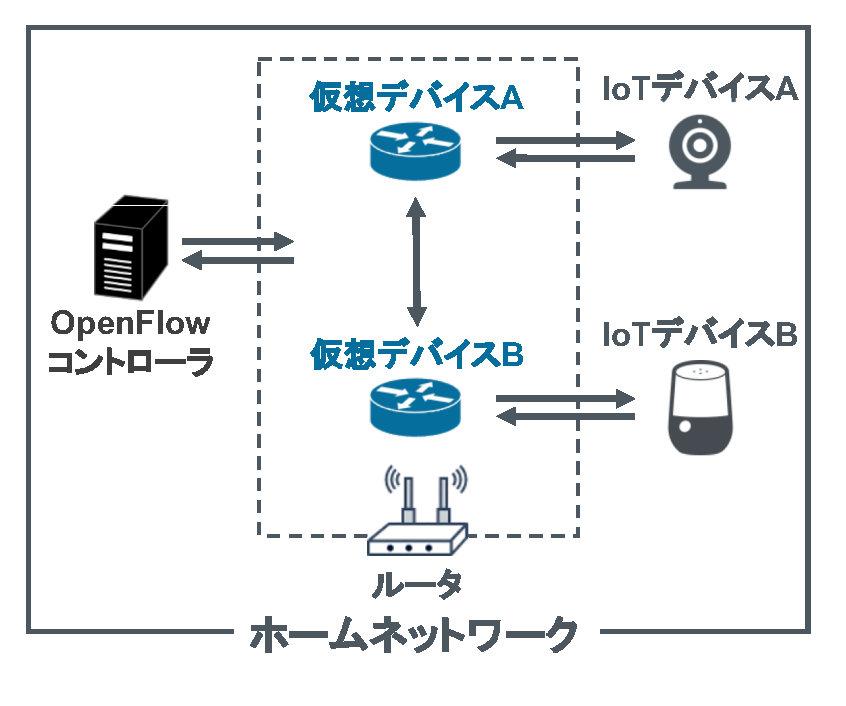
\includegraphics[width=\linewidth]{img/system.eps}
	\caption{提案システムの構成}
	\label{fig:system}
\end{figure}

\section{提案システム}
\subsection{概要}
提案システムでは,セキュリティ対策を適用可能なデバイスをProxyと定義し,ルータ上に仮想的に作成する.
ここに,IoTデバイスがリソース量の制限により適用できないセキュリティ対策をオフロードし,このProxyがIoTデバイス間の通信を中継することで,本来IoTデバイスに適用したいセキュリティ対策を実現する.
また、OpenFlowの機能も追加し、ネットワークの監視を行い、ホームネットワーク内の通信のトラフィック情報は既知であることを考慮し,フローの検証をOpenFlowコントローラで行う.
詳細なセキュリティ対策については後述する.

% 提案システムでは,セキュリティ対策を適用可能なデバイスをProxyと定義し,ルータ上に仮想的に作成する.
% ここに,IoTデバイスがリソース量の制限により適用できないセキュリティ対策をオフロードし,このProxyがIoTデバイス間の通信を中継することで,本来IoTデバイスに適用したいセキュリティ対策を実現する.
% セキュリティ対策として,ホームネットワーク内の通信のトラフィック情報は既知であることを考慮し,フローの検証をOpenFlowコントローラで行う.

\subsection{システム構成}
提案システムの構成を図\ref{fig:system}に示す.本提案システムの構成要素は,IoTデバイス,Proxy,ルータ,仮想環境から構成される.
\begin{itemize}
	\item \underline{IoTデバイス}\mbox{}\\
	      本研究で扱うIoTデバイスは,センサーをはじめとした,CPU等のリソースを十分に保持しておらず,直接セキュリティ対策を適用できないデバイスと定義する.
	\item \underline{Proxy}\mbox{}\\
	      IoTデバイスに要求されるセキュリティ対策を,仮想的に実現したものである.IoTデバイスからの通信を中継し,セキュリティ対策を適用する.セキュリティ対策ごとに作成し,IoTデバイスと紐づけることで,対象デバイスに応じた必要な対策を実現できる.
	\item \underline{ルータ}\mbox{}\\
	      IoTデバイス間通信の中継機器として用いる.ルータ上にコンテナを生成する.
	\item \underline{仮想環境}\mbox{}\\
	      Proxyの実行環境である.Proxyが作成される際に要求されるリソースを十分に提供することが可能である.
\end{itemize}

\begin{figure}[!tb]
	\centering
	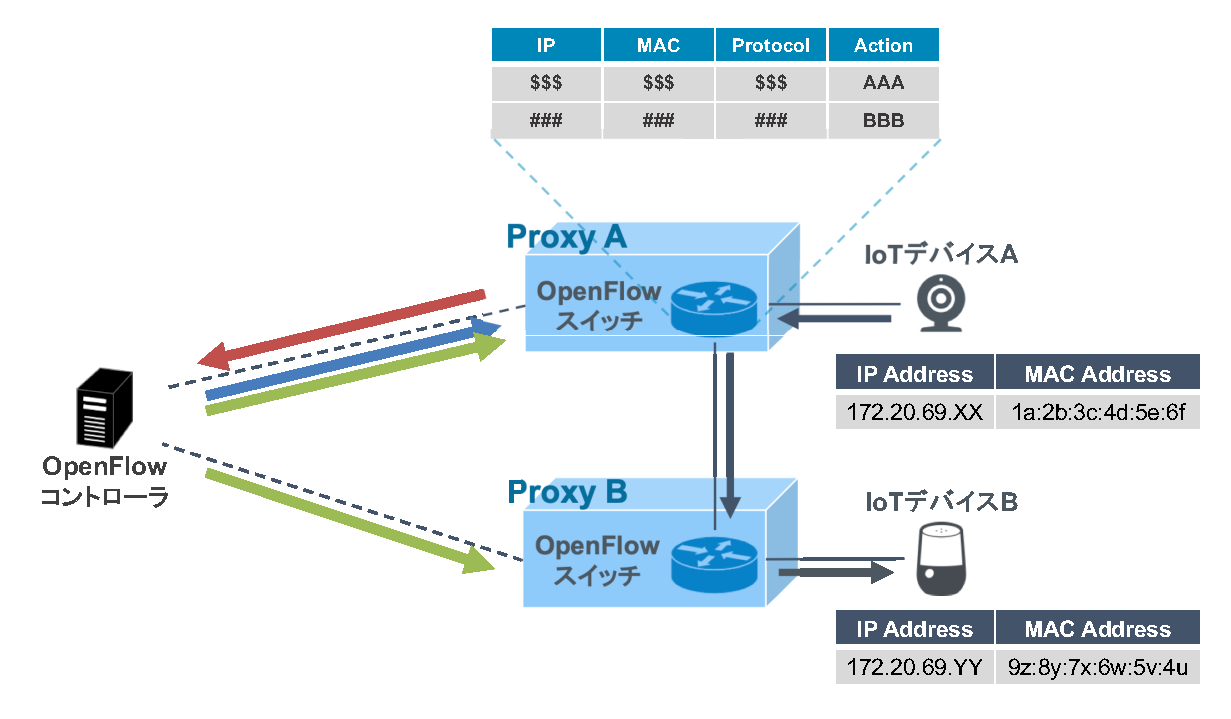
\includegraphics[width=\linewidth]{img/openflow.eps}
	\caption{OpenFlowにおけるフローチェック}
	\label{fig:openflow}
\end{figure}

\subsection{OpenFlowによるフローチェック}
本研究におけるネットワーク監視をOpenFlowを用いて行う.OpenFlowによるフローチェックを図\ref{fig:openflow}に示す.一つのIoTデバイスに対し,Dockerイメージからコンテナ上にOpenFlowスイッチの機能を生成する.IoTデバイスはこのOpenFlowスイッチを中継し,デバイス間通信を行う.OpenFlowコントローラは事前にIoTデバイスの情報を保持しており,デバイス間通信のフローテーブルを作成する.ホームネットワークの特性である各IoTデバイスのトラフィック情報は既知であり、変化が大きくないことを考慮し,IPアドレスや通信頻度の確認を行い,フローレベルにおける攻撃の検知を行う.

\begin{figure}[!tb]
	\centering
	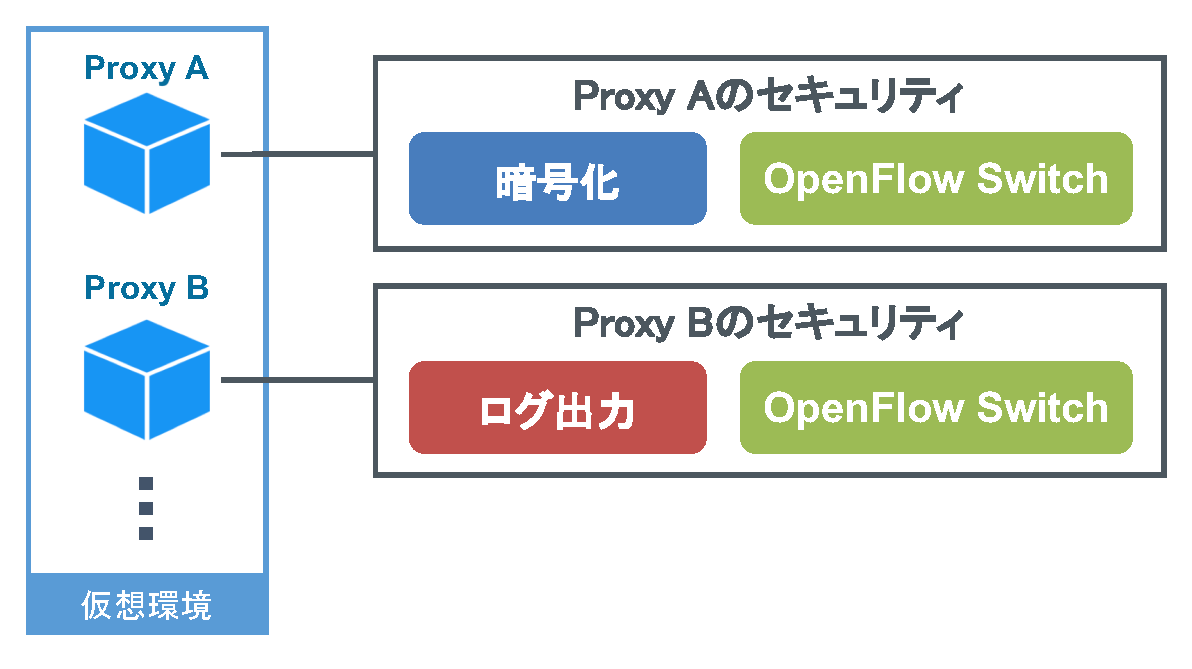
\includegraphics[width=\linewidth]{img/security.eps}
	\caption{Proxyのセキュリティ対策}
	\label{fig:security}
\end{figure}

\begin{figure}[!tb]
	\centering
	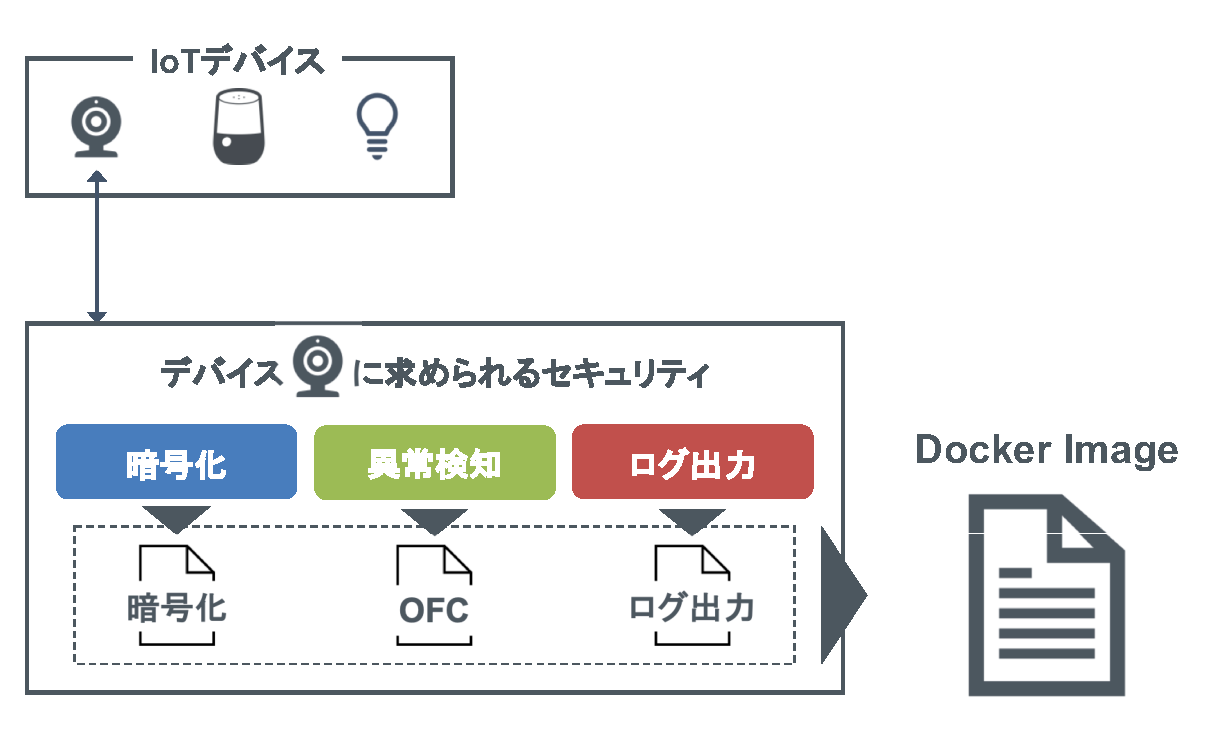
\includegraphics[width=\linewidth]{img/dockerimage.eps}
	\caption{imageファイルの作成}
	\label{fig:dockerimage}
\end{figure}

\subsection{Proxyのセキュリティ対策}
本研究におけるセキュリティ対策の特徴として,Proxyごとに異なるセキュリティ対策を適用可能なことが挙げられる.Proxyのセキュリティ対策の適用例を図\ref{fig:security}に示す.これによりリソースの都合上,IoTデバイスに直接適用できないセキュリティ対策を導入できることに加え,前述のIoTデバイスの問題点で述べたような様々なセキュリティ要件の変更に対しても柔軟に対応が可能となる.\par
また,コンテナ上で展開されるセキュリティ対策は適応したいセキュリティ対策に対応したコンテナのimageファイルで定義される.imageファイルの作成図を図\ref{fig:dockerimage}に示す.この図のようにIoTデバイスに対して適用したいセキュリティが複数ある場合においても,当該デバイスの規格に対応した対策をそれぞれ作成し,ソフトウェアモジュールのような形で組み合わせて定義することで,imageファイルを作成することが可能となる.

\section{実装}
\subsection{実装環境}
本研究の実装環境,実装環境の構成をそれぞれ表\ref{tab:program}と図\ref{fig:program}に示す.Proxyの作成方法としては軽量なアプリケーション実行環境であるDockerを利用した.ProxyをDockerで作成されるコンテナ状で稼働させることで複数のProxyをリソース,オーバーヘッドを抑えて作成できることに加え,Docker Hubより配布されるDocker Imageを用いることで容易に作成可能となる.
% また今回扱う通信プロトコルとしてはhttp(REST)を想定する.

\begin{table}[!bt]
	\caption{実装環境}
	\label{tab:program}
	\centering
	\begin{tabular}{|c|l|l|}
		\hline
		種類     & 項目       & 説明                  \\
		\hline \hline
		Proxy    & 使用ソフト & Docker                \\
		         & OS         & Ubuntu 20.04          \\
		         & CPU        & 3.60GHz Intel Core i9 \\
		         & メモリ     & 5GB                   \\
		\hline
		OpenFlow & 使用ソフト & Ryu                   \\
		         & OS         & Ubuntu 20.04          \\
		         & CPU        & 3.60GHz Intel Core i9 \\
		         & メモリ     & 5GB                   \\
		         & 使用言語   & Python                \\
		\hline
	\end{tabular}
\end{table}

\begin{figure}[!tb]
	\centering
	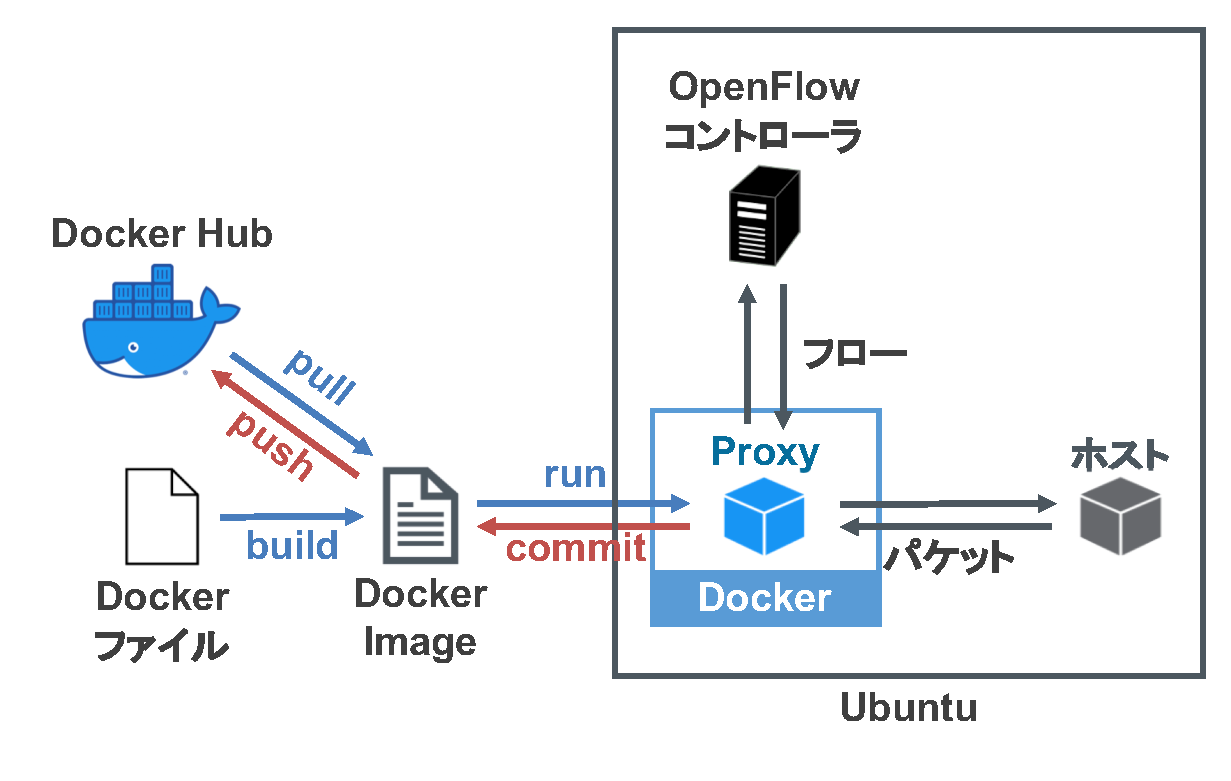
\includegraphics[width=\linewidth]{img/program.eps}
	\caption{実装環境の構成}
	\label{fig:program}
\end{figure}

\subsection{動作手順}
IoTデバイスの所有者であるユーザが本提案システムを利用する際の動作手順を図\ref{fig:seaquence}と以下に示す.
\begin{enumerate}
	\item ユーザはデバイスをLAN内に接続した後,Proxyの受付サーバへアクセス.
	\item Proxyはホームネットワーク内にIoTデバイスが接続されたことを確認.
	\item ProxyはDocker HubからDocker Imageを取得.
	\item 取得したDocker Imageを基に仮想環境内にDocker Imageを作成.
	\item Proxyはデバイス情報を基にIoTデバイスに接続を行い,Proxyを経由して通信を行うように設定.
	\item ProxyはOpenFlowコントローラへデバイス情報を送信.
	\item 設定が完了し,IoTデバイス・Proxy間の通信が確立された後,Proxyの作成・ネットワークの監視状況を報告.
\end{enumerate}


\begin{figure}[!tb]
	\centering
	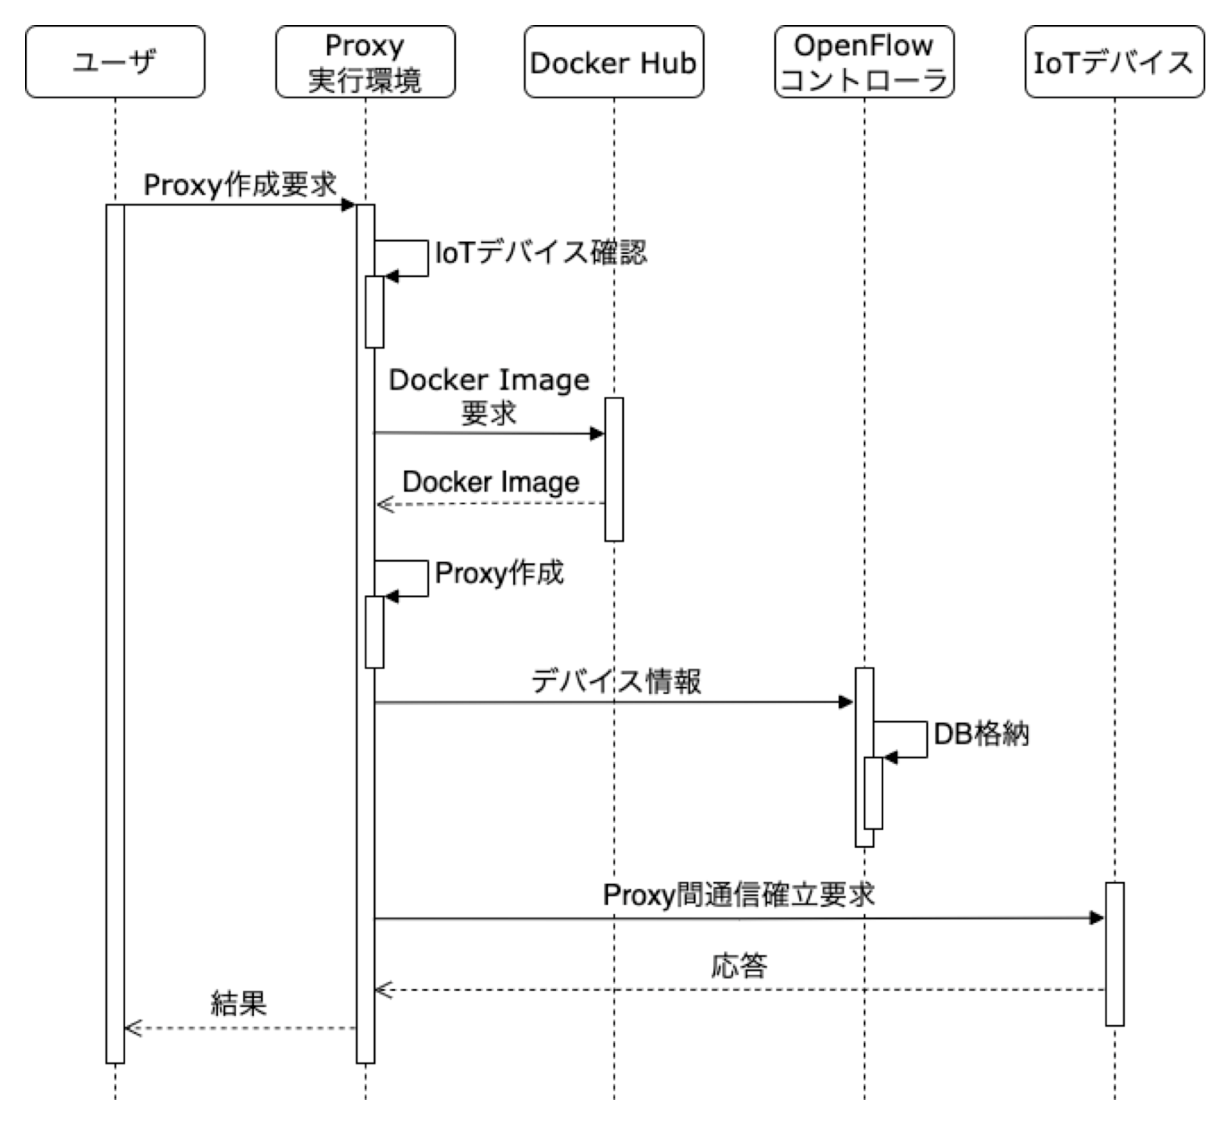
\includegraphics[width=\linewidth]{img/seaquence.eps}
	\caption{動作手順のシーケンス図}
	\label{fig:seaquence}
\end{figure}

\subsection{想定ユースケース}
本提案システムを用いた想定ユースケースを以下に示す.各DockerイメージはDocker Hubというユーザが作成したコンテナをアップロードして公開・共有できるサービスを利用することを想定する.

\begin{itemize}
	\item \underline{セキュリティ対策をあらかじめ提供する場合}\mbox{}\\
	      SSLによる通信の暗号化など,IoTデバイスのリソースを多く利用するために適用できないセキュリティ対策をあらかじめDockerイメージとして提供し,Proxy上で実現する.
	\item \underline{インシデント発生時などに対策を提供する場合}\mbox{}\\
	      事前に提供していたセキュリティ対策では想定していなかったインシデント等が発生した場合等に,当該デバイスの持つリソース量に依存せず,追加のセキュリティ対策を提供することが可能となる.
\end{itemize}

\begin{figure*}[!tb]
	\centering
	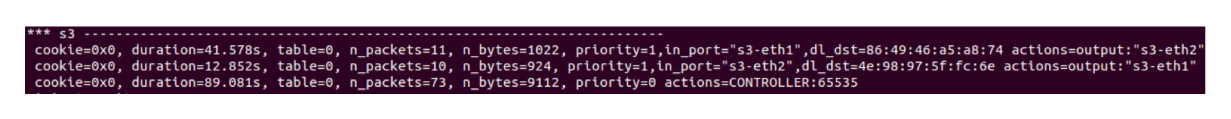
\includegraphics[width=\linewidth]{img/result_flow4v2.eps}
	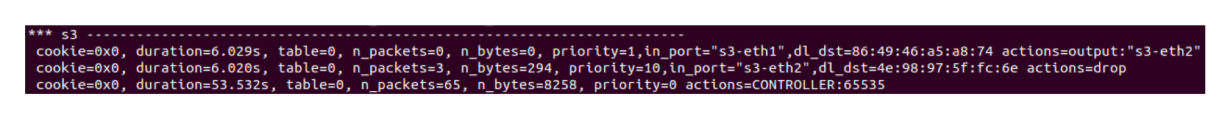
\includegraphics[width=\linewidth]{img/result_flow2v2.eps}
	
\includegraphics[width=\linewidth]{img/result_flow3v2.eps}
	\caption{登録済みのホストのフローテーブル(上),異常時のパケットをDrop処理するフローテーブル(中),その後のアクションが削除されたフローテーブル(下)}
	\label{fig:result1}
\end{figure*}

\section{評価}
\subsection{評価内容}
本研究の評価として,まずセキュリティが適用されているかを検証した.今回は存在を把握していないIoTデバイスから通信があった場合と、あるデイバイスからの通信頻度が通常と異なる場合を想定した.それに対し,OpenFlowによるフローチェックが行われているかを検証した.\par
また,提案システムを適用した上で,IoTデバイス間で通信した際のEndtoEndの時間を計測を行った.比較対象として,セキュリティ対策を適用せず、ルータを経由してデバイス間通信を行う場合についても計測を行った.

\subsection{評価環境}
今回適用するセキュリティ対策としては,鍵長が1024bitのSSLによる暗号化のイメージをDocker Hubより取得し,適用した.また,OpenFlowスイッチのイメージも取得し,OpenFlowによるフローチェックも行った.

\section{結果と考察}

% \begin{figure}[!tb]
% 	\centering
% 	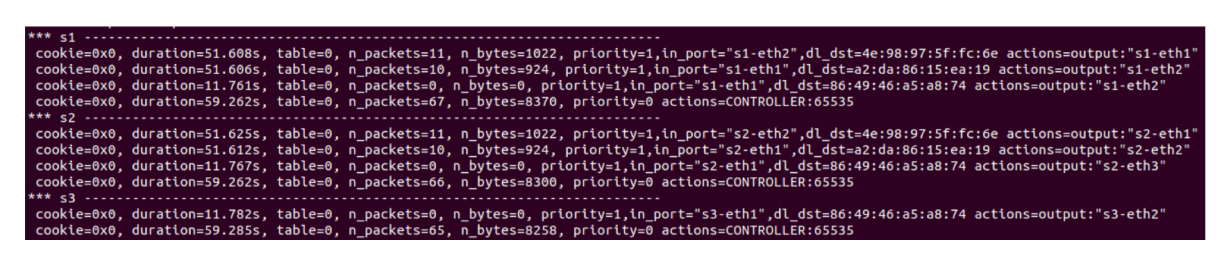
\includegraphics[width=\linewidth]{img/result_flow3.eps}
% 	\caption{imageファイルの作成}
% 	\label{fig:result2}
% \end{figure}

% \begin{figure}[!tb]
% 	\centering
% 	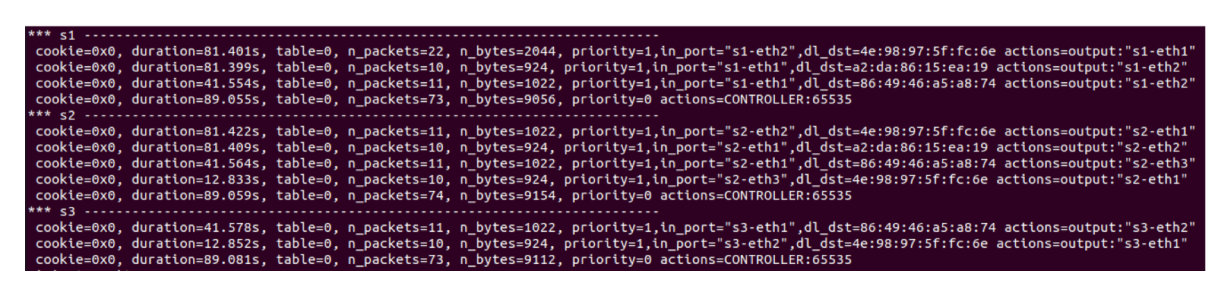
\includegraphics[width=\linewidth]{img/result_flow4.eps}
% 	\caption{imageファイルの作成}
% 	\label{fig:result3}
% \end{figure}

\subsection{評価結果}
登録済みのIoTデバイスかた通信要求が来た場合,登録していないIoTデバイスや通常の通信頻度と異なる等の異常の通信がなされている場合のフローテーブルの結果を図\ref{fig:result1}に示す.通常時は他のデバイスに対し,フローテーブルが作成されているが,異常時はパケットをDrop処理するフローテーブルが作成されており,その後、そのフローテーブルが削除されていることがわかる.\par
また,セキュリティ対策を施した提案システムとセキュリティ対策を施してないシステムにおける通信の比較結果を図に示す.

\subsection{信頼性に関する考察}
IoTデバイスを用いたシステムの安心安全を確保するための機能として,IPAによりIoT高信頼化昨日が定義されており,IoT高信頼化要件として,IPAによりIoT高信頼化要件として,開始,予防,検知,回復,終了の5つの局面に分けてそれぞれセキュリティ要件が定義されている\cite{IPA}.今回は前述の5つより,システム稼働中の局面である予防,検知,回復の3つにおける高信頼化要件に対し,提案システムの有効性について考察する.

\begin{itemize}
	\item \underline{予防の局面における考察}\mbox{}\\
	      予防の局面での高信頼化要件は,稼働中の異常発生を未然に防止できることである.これに対応するIoT高信頼化機能としては,ログ取集機能,暗号化機能等があり,以上の予兆の把握,資産の保護を実現する.提案システムを用いることで,リソース量の関係で通常のIoTデバイスに適用できない機能であっても適用可能となる.
	\item \underline{検知の局面における考察}\mbox{}\\
	      検知の局面での高信頼化要件は,稼働中の異常発生を早期に検知できることである.これに対応するIoT高信頼化機能としては,OpenFlowによるネットワーク監視機能,ログ収集機能があり,以上発生の検知や発生原因の特定を実現する.提案システムを用いることで,予防の局面同様,デバイスのリソース量に依存せず,求められる機能を実現できることに加え,Proxyは各IoTデバイスごとに作成するため,個々のデバイスに応じた詳細な検知ルールを適用可能となる.
	\item \underline{回復の局面における考察}\mbox{}\\
	      回復の局面での高信頼化要件は,異常が発生した場合に稼働の復旧ができることである.特にIoTでは,さまざまなデバイスが相互通信を行うため,事前に予測していなかった異常が発生することが考えられる.今回の環境では各セキュリティ対策はDocker Hubを通してDockerイメージとして提供することで,事前に作成したセキュリティ対策だけでなく,追加のセキュリティ対策も配布・適用が容易である.
\end{itemize}

\subsection{性能に関する考察}
図より、本提案システムであるDockerを用いたProxyによるセキュリティ対策、OpenFlowによるネットワーク監視は、セキュリティ対策なしの場合と比較し遅延は発生しているが、許容範囲内であり、実用性があると考えられる.\par
今後IoTデバイスが普及した際には、クラウドへの通信量が爆発的に増加するため、帯域の輻輳といった問題も発生すると考えられる.そのため、通信遅延はさらに増加することが想定されることから、通信遅延が許容が難しいアプリケーションを利用する際にセキュリティ対策が必要な場合には本提案システムが有効となる.

\section{まとめ}
近年,IoT(Internet of Things)が注目を集めるようになり,今後あらゆるモノがネットワークに接続され,利用されることが予想される.しかし,IoTの発展により利便性が高まる一方で,これまでネットワークに接続されていなかったモノが接続されることにより,セキュリティ上のリスクも高まっている.また,今後はホームネットワーク内で閉じたデバイス間の通信によって連携を行う形になることが想定される.デバイス間で直接通信を行う場合,各デバイスにおいてどのデバイスとの通信を受け入れるか,アクセス制御を行う必要がある.そこで本研究では,SDN(Software Defined Networks)の代表的プロトコルであるOpenFlowを用いて,ホームネットワーク内の通信を監視するフレームワークの構築を検討した.また,提案システムでは,セキュリティ対策をオフロードしたProxyを仮想的に作成し.IoTデバイス間の通信を中継することで,本来IoTデバイスに適用したいセキュリティ対策を実現した.そして,IoTデバイス間で閉じた通信を行うシミュレーション評価の比較より,ホームネットワークにおいてセキュリティ要件を保つことと性能も許容範囲であることを示した.\par
今後は,オーケストレータ等を用いて,新しいIoTデバイスがホームネットワークに追加された際に,自動的にコンテナがProxyとして配備される仕組みを検討する.また,Raspberry Pi等の実機を用いた実験を行う予定である.

\begin{thebibliography}{10}
	\bibitem{security} 総務省,"IoT・5Gセキュリティ総合対策2020", サイバーセキュリティタスクフォース, pp.1-56, 2020.
	\bibitem{lowcost} A. Sivanathan, D. Sherratt, H. H. Gharakheili, V. Sivaraman and A. Vishwanath, "Low-cost flow-based security solutions for smart-home IoT devices," 2016 IEEE International Conference on Advanced Networks and Telecommunications Systems (ANTS), pp.1-6, 2016.
	\bibitem{d2d} C. Vallati et al., "Mobile-Edge Computing Come Home Connecting things in future smart homes using LTE device-to-device communications", IEEE Consumer Electronics Magazine, Vol.5, No.4, pp.77-83, 2016.
	\bibitem{disap} M. Serror et al., "Towards In-Network Security for Smart Homes", Proceedings of the 13th International Conference on Availability, Reliability and Security (ARES 2018), No.18, pp.1-8, 2018.
	\bibitem{sover} Z. Zhang, T. Yu, X. Ma, Y. Guan, P. Moll and L. Zhang, "Sovereign: Self-contained Smart Home with Data-centric Network and Security", IEEE Internet of Things Journal, 2022.
	\bibitem{openflow} Nick McKeown et al., "OpenFlow: enabling innovation in campus networks", SIGCOMM Computer Communication Review, Vol.38, pp.69–74, 2008.
	\bibitem{IPA} IPA技術本部 ソフトウェア高信頼化センター(SEC), "「つながる世界の開発指針」の実践に向けた手引き", 2017.
\end{thebibliography}

\end{document}
